\chapter{AI Model for Romanian Language}
\label{chap:ch4}
\par \quad Multilingual depression detection is highly dependant on the capability of AI models to understand and analyze text from different cultures. This section describes the process of translating English text into Romanian, a step essential for training our AI model to recognize depressive patterns in a multilingual context. We will discuss the selection criteria and the impact of utilizing a specific Translation API to bridge the language gap, thus enabling our model to process and interpret Romanian text with the same level of accuracy as English. 

\section{Reasoning Behind Choosing Yandex}

\quad In our effort to refine our multilingual depression detection model, we referenced a detailed study that assessed the efficiency, accuracy, and security of various Translation APIs \cite{rashmi2020comparison}. This comparative analysis served as the foundation for selecting the most suitable API for our application, which required the translation of text from English to Romanian among other language pairs. The study meticulously compared several leading Translation APIs, including Google API, Microsoft, Systran.io, MyMemory, and Yandex, focusing on their performance in terms of speed, accuracy, security, and the breadth of language support.
\begin{itemize}
\item \textbf{Google API} is widely recognized for its impressive language support, capable of translating content across more than 100 languages. This extensive reach makes it a versatile tool for global communication and content translation. Its reputation and prevalence in the market are testaments to its utility and user-friendly interface. Additionally, it's worth noting that while Google API is commendable, it is not a free service, which may affect its accessibility for some users.\cite{rashmi2020comparison}.

\item \textbf{Microsoft's Translation API} is lauded for its quality and security, offering translations among 60+ languages. It stands out for its emphasis on accuracy and stringent security protocols, although its language support is less extensive than Google's \cite{rashmi2020comparison}.

\item \textbf{Systran.io} boasts a high accuracy rate of 99\%, albeit with limitations in recognizing slang, nuances, and culturally relevant phrases. Its security is commendable, positioning it as a reliable choice for many applications \cite{rashmi2020comparison}.

\item \textbf{MyMemory} excels in translation speed but experiences the highest latency among the APIs evaluated. While it supports translations between 80+ languages, the absence of training data for certain language combinations limits its effectiveness. Nonetheless, its security is robust \cite{rashmi2020comparison}.

\item \textbf{Yandex API}, with support for 90+ languages, stands out for its balance of translation accuracy and lower latency compared to its counterparts. Despite its efficiency and broad language coverage, its security features are not optimal for translating confidential documents \cite{rashmi2020comparison}.
\end{itemize}

The conclusion from this study discussed the strengths and weaknesses of each API, guiding our choice towards Yandex API for our multilingual depression detection model. Yandex was selected due to its free access, lower latency, and reliable accuracy across different cultures, making it an ideal tool for everyday translations where security is not the biggest concern \cite{rashmi2020comparison}. This choice aligns with our objective of giving people an easy to use and accessible tool in order to prevent problems that could appear with depression.

Another rigorous study \cite{cambedda2021study} provides a nuanced error analysis of Yandex's translations. Notably, Yandex's performance, depicted in the graph \ref{YandexTranslationPerformance}, indicates a relatively uniform distribution of errors across multiple categories. This suggests that while Yandex does have areas where it lacks consitency, such as Lexis, Syntax, and Article Usage, it generally maintains the core meaning of the translated text. This is critical for our model, which relies on emotion categories to accurately detect depression in text.

\begin{figure}[htbp]
	\centering
		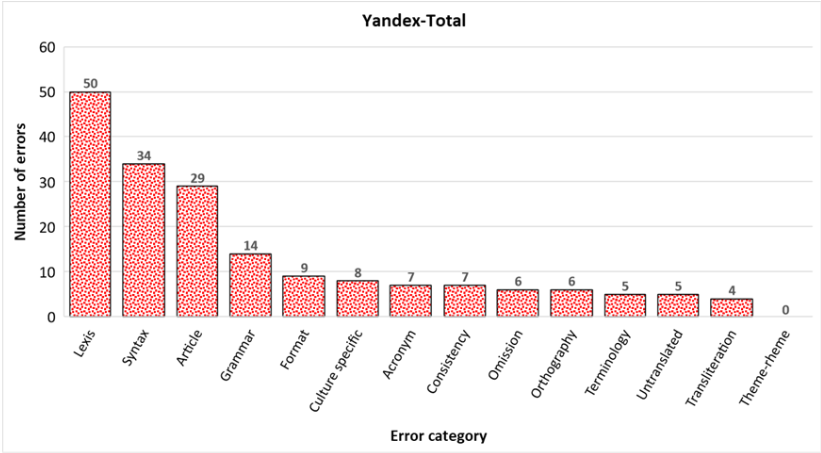
\includegraphics[scale=0.65]{LaTeX Bachelor Thesis Depression Signs Detection/figures/Yandex's-translation-performace.png}
	\caption{Yandex's translation performance \cite{cambedda2021study}}
	\label{YandexTranslationPerformance}
\end{figure}

The Lexis category, in particular, displays the highest number of errors, signaling a need for further investigation to understand whether these issues are from the nature of the texts or from challenges within the translation tool. However, it is encouraging to note that error categories such as Grammar, Format, Culture-Specific References, Acronym, and Consistency show significantly fewer errors. These categories are essential for maintaining the general meaning, which reaffirms our choice of Yandex for texts where nuanced meaning is less likely to affect the detection of depression signs.

Further examination of the study indicates that Yandex demonstrates a more adept handling of common language texts as opposed to those with specialized jargon, registering fewer errors in translations of texts with language spoken by the people in a particular country or region \cite{cambedda2021study}. Considering our dataset comprises of Reddit posts, which are typically phrased in everyday language, this finding is particularly relevant. The study also highlights that, with the exception of Article Usage, the disparity in error rates between different text types is negligible, suggesting that Yandex can reliably manage the conversational and informal style characteristic of Reddit communications.

\section{Adjusting to Yandex API's Policy Shift}

\quad We had initially recognized the Yandex API as a superior option, particularly for its cost-effectiveness, as it was freely accessible at the time of study \cite{rashmi2020comparison}. This advantage aligned with our objectives, allowing us to use its translation capabilities without financial constraints.

However, since the publication of \cite{rashmi2020comparison}, Yandex's policy has undergone significant changes. The API, once free to use within a given generous limit, now requires users to possess a registered and legally recognized company to utilize its services. Ihe requirement of company registration introduces a barrier, limiting the accessibility of Yandex API for independent researchers, small teams, or educational institutions.

Given these new rules, we are still fully dedicated to creating a useful and easy-to-use depression detection system that works in many languages. Therefore, we are looking into different approaches.

\section{Shifting to googletrans}

\quad We decided to integrate the googletrans library \cite{googletranslib} into our multilingual depression detection model. It offers a free and unlimited Python library that uses the Google Translate API. This library appears particularly advantageous for our requirements, as it is not only accessible without cost but also does not require the a company registration that Yandex now demands. As it can be seen in \ref{codeGoogleTransUsage}, it is very accessible to translate text in Python from English ro Romanian.

\begin{figure}[htbp]
	\centering
		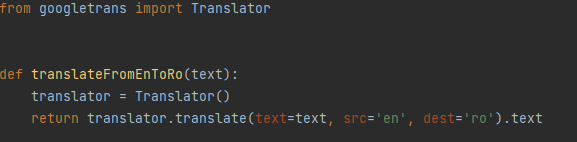
\includegraphics[scale=1]{LaTeX Bachelor Thesis Depression Signs Detection/figures/codeGoogleTransUsage.png}
	\caption{Python library "googletrans" translation from English to Romanian}
	\label{codeGoogleTransUsage}
\end{figure}

The googletrans library \cite{googletranslib} has features that are well-suited to our project's needs. It is recognized for its speed and reliability, as it operates on the same servers as translate.google.com. The library supports auto language detection, facilitating the identification and translation of a wide array of languages without prior specification. Additionally, it provides the capability for bulk translations, which is invaluable when processing large datasets typically found in NLP tasks. It was done for the chosen dataset \cite{depressionDataset} in Python as it can be seen in \ref{codeDatasetTranslation} .

\begin{figure}[htbp]
	\centering
		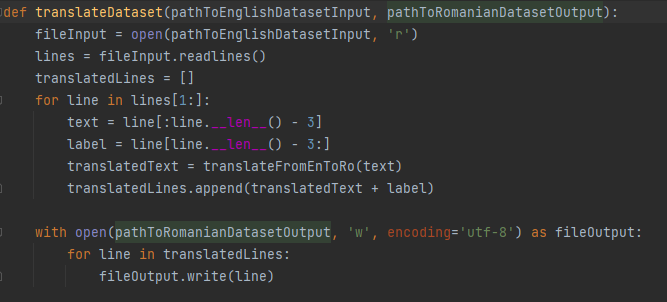
\includegraphics[scale=1]{LaTeX Bachelor Thesis Depression Signs Detection/figures/codeDatasetTranslation.png}
	\caption{Python code for translating dataset from English to Romanian}
	\label{codeDatasetTranslation}
\end{figure}

It is also important to acknowledge googletrans's \cite{googletranslib} usage notes. The 15,000-character limit per text may require segmentation of longer entries, and the instability of web-based translation services means that we should proceed with precaution regarding the library's reliability. The developers themselves suggest opting for the official Google Translate API for more advanced applications where stability is very important. Furthermore, potential HTTP errors could indicate temporary bans by Google, meaning that it is needed to keep an eye on and manage how we use our API to avoid any interruptions. Despite these considerations, the googletrans library's free and flexible usage makes it an excellent fit for our project in its current stage.

\section{Model Training}

\quad For the Romanian language model, the methodology was replicated consistently. LIWC served as the tool for preprocessing the data. However, the most recent English dictionary for LIWC-22 has not been translated into Romanian. The latest available version for Romanian is the LIWC-2015 dictionary, which contains only 86 features, compared to the 119 features available in the English version.

The training approach was aligned with the methodology used for the English model during the second experiment. The hyperparameters and the proportion of training to testing data remain consistent:

\begin{itemize}
\item \textbf{train/test split}: Maintained at 75/25, using stratification based on the 'is\_depression' label
\item \textbf{mtry}: 6
\item \textbf{Number of trees}: 900
\item \textbf{Node Size}: 3
\item \textbf{Sample size}: 8
\end{itemize}

This methodology facilitates a direct comparison between the performance of the Romanian and English models, ensuring consistent evaluation criteria across both. The same metrics were used for analysis. In terms of classification metrics, the most notable discrepancy arises in recall, where the Romanian model scores 0.87, falling short of the English model's 0.96 by 9 percentage points. Additionally, both accuracy and the F1-score have diminished by 0.05, while precision experienced the least impact, decreasing from 0.99 to 0.97. These metrics are illustrated in Figure \ref{classificationMetricsSecondExperiment} for the English model and in Figure \ref{classificationMetricsRomanianExperiment} for the Romanian model.

The diminished recall in the Romanian model suggests it is less adept at identifying true positive cases as compared to the English model. This lower performance may come from the nuances lost during the translation of the dataset from English to Romanian using the Googletrans library \cite{googletranslib}. Such translation challenges could contribute to the model’s reduced effectiveness, highlighting the influence of linguistic or cultural differences on the model’s ability to generalize across languages. The smaller reductions in accuracy and F1-score indicate that while the model is somewhat less effective overall, it still maintains a reasonable level of precision.

\begin{figure}[htbp]
	\centering
		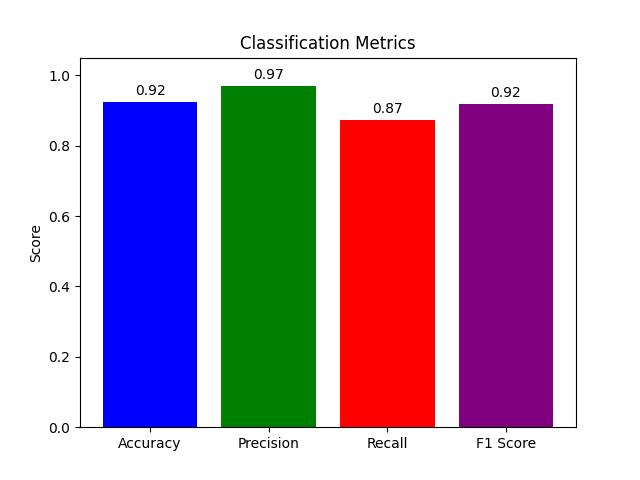
\includegraphics[scale=0.8]{LaTeX Bachelor Thesis Depression Signs Detection/figures/metrics/experimentRomanian/classificationMetrics.jpg}
	\caption{Classification Metrics Romanian Model}
	\label{classificationMetricsRomanianExperiment}
\end{figure}

The confusion matrix \ref{confusionMatrixRomanianExperiment} illustrates a significant increase in false positives, rising from 43 in the English model \ref{confusionMatriSecondExperiment} to 123 in the Romanian model. However, the rise in false negatives was less marked, increasing from 7 to 26.

\begin{figure}[htbp]
	\centering
		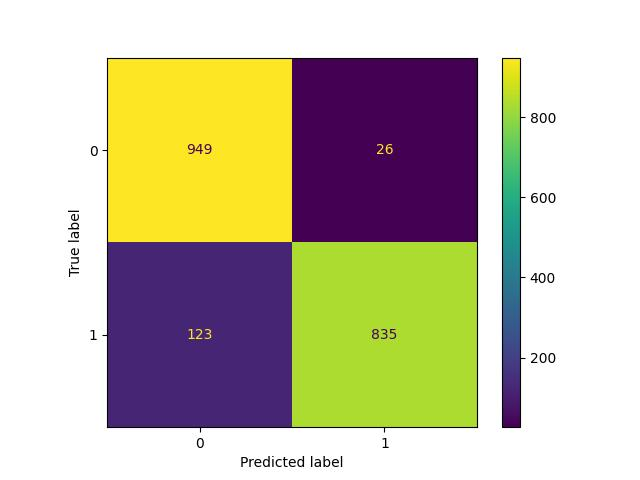
\includegraphics[scale=0.8]{LaTeX Bachelor Thesis Depression Signs Detection/figures/metrics/experimentRomanian/confusionMatrix.jpg}
	\caption{Confusion Matrix Romanian Model}
	\label{confusionMatrixRomanianExperiment}
\end{figure}

Regarding the ROC curve, the Area Under the Curve (AUC) experienced a slight decrease of 0.01, as depicted in Figure \ref{rocCurveRomanianExperiment} compared to Figure \ref{rocCurveSecondExperiment}. These metrics collectively indicate that the issues observed during the experimentation with the English model are more pronounced in the Romanian classifier.

\begin{figure}[htbp]
	\centering
		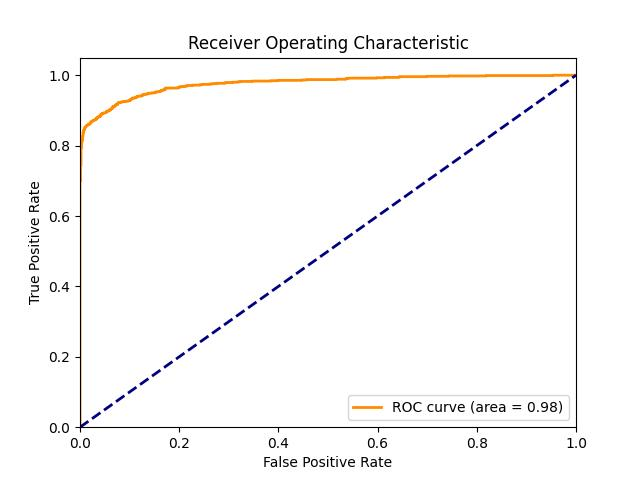
\includegraphics[scale=0.8]{LaTeX Bachelor Thesis Depression Signs Detection/figures/metrics/experimentRomanian/roc_curve.jpg}
	\caption{ROC Curve Romanian Model}
	\label{rocCurveRomanianExperiment}
\end{figure}

The most significant features for the Romanian classifier \ref{top10FeaturesRomanianExperiment} align more closely with those observed in the initial experiment for the English model \ref{top10FeaturesFirstExperiment}. Notably, Word Count (WC) has risen above 0.12, surpassing the prominence it held in the first experiment. This contrasts with the enhancements seen in the second English experiment \ref{top10FeaturesSecondExperiment}, where a diminished reliance on WC and WPS (Words per Sentence) indicated a broader array of features influencing the English classifier’s decisions. However, this diversification does not appear to extend to the Romanian model.

Some features remain consistent with the English LIWC-22 dictionary features listed in the top 10 for the second experiment; for instance, "sad" aligns with "emo\_sad", and both "cause" and "health" are both present and "negemo" is the same as "emo\_neg". The "anx" feature mirrors "emo\_anx" from the first experiment’s top features. The presence of "Period" suggests that the Googletrans library has introduced punctuation marks, which have become a significant element. The evolution from LIWC-2015 to LIWC-22 is further evidenced by the removal of the "interrog" category in the Romanian model’s top 10 features, which was dropped in LIWC-22 due to its low base rates, internal reliability, or infrequent usage, as noted in \cite{boyd2022development}. The "ipron" feature might also result from the machine translation process.

\begin{figure}[htbp]
	\centering
		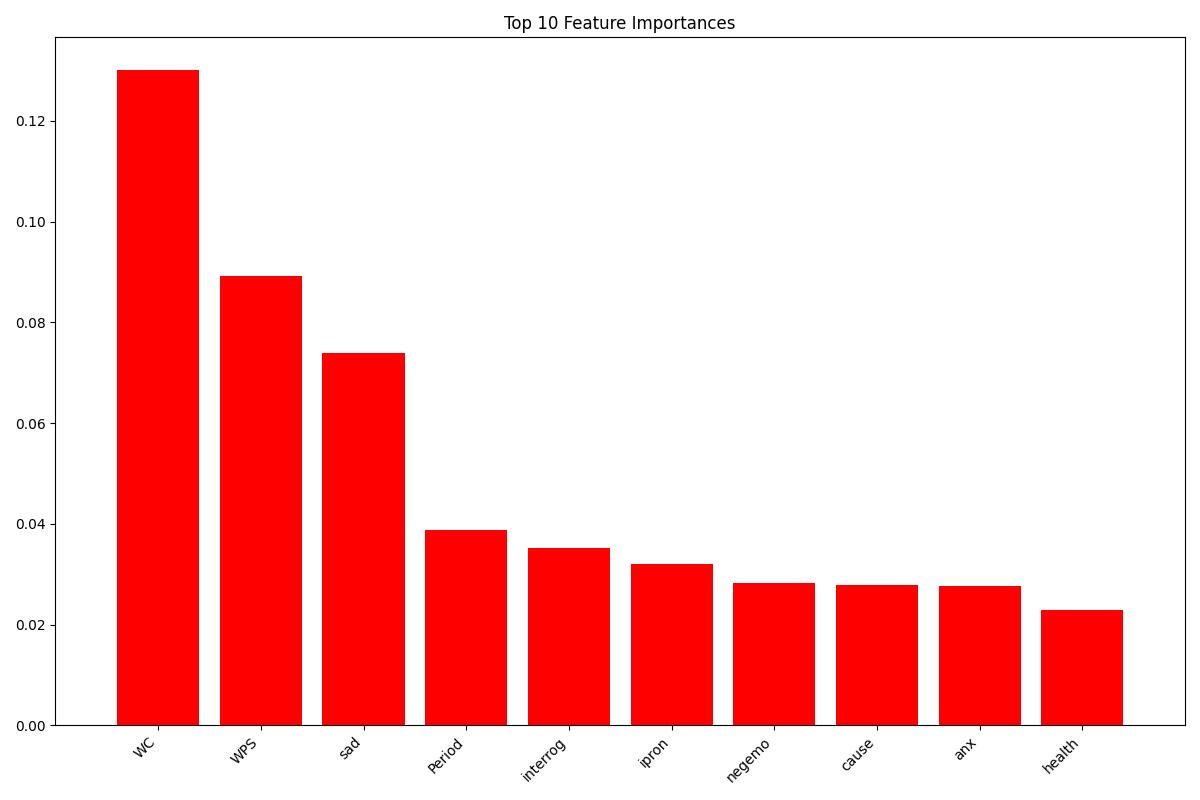
\includegraphics[scale=0.5]{LaTeX Bachelor Thesis Depression Signs Detection/figures/metrics/experimentRomanian/top10features.jpg}
	\caption{Top 10 Features Romanian Model}
	\label{top10FeaturesRomanianExperiment}
\end{figure}